\documentclass[portrait,a0,final]{a0poster}

% Fonts
\usepackage{fontspec}
\setmainfont[
  Path=./fonts/PT_Sans/,
  BoldFont={PT_Sans-Web-Bold},
  ItalicFont={PT_Sans-Web-Italic},
  BoldItalicFont={PT_Sans-Web-BoldItalic}
]{PT_Sans-Web-Regular.ttf}

% Colors and colour gradients
\usepackage{xcolor,colortbl}

% Palettes from: https://betterfigures.org/2015/06/23/picking-a-colour-scale-for-scientific-graphics/
% Greys:
\definecolor{grey0}{rgb}{1.0,1.0,1.0} % White
\definecolor{grey1}{rgb}{0.94,0.94,0.94}
\definecolor{grey2}{rgb}{0.85,0.85,0.85}
\definecolor{grey3}{rgb}{0.74,0.74,0.74}
\definecolor{grey4}{rgb}{0.59,0.59,0.59}
\definecolor{grey5}{rgb}{0.45,0.45,0.45}
\definecolor{grey6}{rgb}{0.32,0.32,0.32}
\definecolor{grey7}{rgb}{0.15,0.15,0.15}
\definecolor{grey8}{rgb}{0.0,0.0,0.0} % Black

% Blues:
\definecolor{blue0}{rgb}{0.97,0.98,1.0}
\definecolor{blue1}{rgb}{0.87,0.93,0.97}
\definecolor{blue2}{rgb}{0.78,0.86,0.94}
\definecolor{blue3}{rgb}{0.62,0.79,0.88}
\definecolor{blue4}{rgb}{0.42,0.68,0.84}
\definecolor{blue5}{rgb}{0.26,0.57,0.78}
\definecolor{blue6}{rgb}{0.13,0.44,0.71}
\definecolor{blue7}{rgb}{0.03,0.32,0.61}
\definecolor{blue8}{rgb}{0.03,0.19,0.42}

% Yellow-Green-Blue:
\definecolor{YlGnBu0}{rgb}{1.0,1.0,0.85}
\definecolor{YlGnBu1}{rgb}{0.93,0.98,0.69}
\definecolor{YlGnBu2}{rgb}{0.78,0.91,0.71}
\definecolor{YlGnBu3}{rgb}{0.50,0.80,0.73}
\definecolor{YlGnBu4}{rgb}{0.25,0.71,0.77}
\definecolor{YlGnBu5}{rgb}{0.11,0.57,0.75}
\definecolor{YlGnBu6}{rgb}{0.13,0.37,0.66}
\definecolor{YlGnBu7}{rgb}{0.15,0.20,0.58}
\definecolor{YlGnBu8}{rgb}{0.03,0.11,0.35}

% Yellow-Orange-Red:
\definecolor{YlOrRd0}{rgb}{1.0,1.0,0.8}
\definecolor{YlOrRd1}{rgb}{1.0,0.93,0.63}
\definecolor{YlOrRd2}{rgb}{1.0,0.85,0.46}
\definecolor{YlOrRd3}{rgb}{1.0,0.70,0.30}
\definecolor{YlOrRd4}{rgb}{0.99,0.55,0.24}
\definecolor{YlOrRd5}{rgb}{0.99,0.31,0.16}
\definecolor{YlOrRd6}{rgb}{0.89,0.10,0.11}
\definecolor{YlOrRd7}{rgb}{0.74,0.0,0.15}
\definecolor{YlOrRd8}{rgb}{0.50,0.0,0.15}

% Palettes from: https://digitalsynopsis.com/design/minimal-web-color-palettes-combination-hex-code/
% 1:
\definecolor{RoseBud0}{rgb}{0.98,0.70,0.58}
\definecolor{RoseBud1}{rgb}{0.95,0.45,0.50}
\definecolor{RoseBud2}{rgb}{0.76,0.42,0.53}
\definecolor{RoseBud3}{rgb}{0.43,0.36,0.49}
\definecolor{RoseBud4}{rgb}{0.20,0.36,0.49}

% 2:
\definecolor{Norway0}{rgb}{0.60,0.73,0.60}
\definecolor{Norway1}{rgb}{0.99,0.81,0.67}
\definecolor{Norway2}{rgb}{0.96,0.51,0.49}
\definecolor{Norway3}{rgb}{0.92,0.29,0.38}
\definecolor{Norway4}{rgb}{0.15,0.21,0.23}

% 3:
\definecolor{Padua0}{rgb}{0.68,0.86,0.78}
\definecolor{Padua1}{rgb}{0.86,0.93,0.76}
\definecolor{Padua2}{rgb}{1.0,0.82,0.71}
\definecolor{Padua3}{rgb}{0.97,0.65,0.65}
\definecolor{Padua4}{rgb}{0.96,0.54,0.58}

% 4:
\definecolor{SilverChalice0}{rgb}{0.66,0.65,0.66}
\definecolor{SilverChalice1}{rgb}{0.80,0.33,0.49}
\definecolor{SilverChalice2}{rgb}{0.92,0.09,0.37}
\definecolor{SilverChalice3}{rgb}{0.29,0.29,0.29}
\definecolor{SilverChalice4}{rgb}{0.21,0.21,0.21}

% 5:
\definecolor{Hibiscus0}{rgb}{0.66,0.13,0.42}
\definecolor{Hibiscus1}{rgb}{0.92,0.11,0.30}
\definecolor{Hibiscus2}{rgb}{0.95,0.42,0.27}
\definecolor{Hibiscus3}{rgb}{0.96,0.86,0.41}
\definecolor{Hibiscus4}{rgb}{0.18,0.59,0.60}

% 6:
\definecolor{Tusk0}{rgb}{0.88,0.93,0.76}
\definecolor{Tusk1}{rgb}{0.93,0.90,0.45}
\definecolor{Tusk2}{rgb}{0.97,0.83,0.13}
\definecolor{Tusk3}{rgb}{0.96,0.56,0.24}
\definecolor{Tusk4}{rgb}{0.94,0.31,0.33}

% 7:
\definecolor{Mimosa0}{rgb}{0.90,0.94,0.76}
\definecolor{Mimosa1}{rgb}{0.64,0.84,0.67}
\definecolor{Mimosa2}{rgb}{0.23,0.69,0.66}
\definecolor{Mimosa3}{rgb}{0.33,0.49,0.51}
\definecolor{Mimosa4}{rgb}{0.36,0.32,0.31}

% 8:
\definecolor{RadicalRed0}{rgb}{0.94,0.27,0.40}
\definecolor{RadicalRed1}{rgb}{0.96,0.61,0.60}
\definecolor{RadicalRed2}{rgb}{0.98,0.81,0.68}
\definecolor{RadicalRed3}{rgb}{0.78,0.78,0.67}
\definecolor{RadicalRed4}{rgb}{0.52,0.61,0.61}


% Graphics
\usepackage{graphicx}
\graphicspath{
  {./assets/}
}

% Geometry
\usepackage{geometry}
\geometry{
  left=20mm,
  top=20mm,
  right=20mm,
  bottom=20mm
}

% PS line and shape drawing
\usepackage{tikz}

% Array package
\usepackage{array}
\newcolumntype{C}[1]{>{\centering\let\newline\\\arraybackslash\hspace{0pt}}m{#1}}
\newcolumntype{L}[1]{>{\raggedright\let\newline\\\arraybackslash\hspace{0pt}}m{#1}}
\newcolumntype{R}[1]{>{\raggedleft\let\newline\\\arraybackslash\hspace{0pt}}m{#1}}
\setlength{\tabcolsep}{0.1\linewidth}

% Wrapping text around figures
\usepackage{wrapfig}

% Math
\usepackage{unicode-math}

% Multirow
\usepackage{multirow}

% Line control (spacing, ...)
\usepackage{setspace}
\renewcommand{\baselinestretch}{1}

% Boxes
\usepackage{adjustbox}
\newlength{\strutheight}

% New commands
\newcommand{\mc}[3]{\multicolumn{#1}{#2}{#3}}
\newcommand{\mr}[2]{\multirow{#1}{*}{#2}}
\newcommand{\wtxt}[1]{{\color{grey0} #1}} % White text
\newcommand{\gtxt}[1]{{\color{grey6} #1}}

% New environments
% Section: section{picture}{title}{subtitle}
\renewenvironment{section}[3]
{
\vspace{2cm}
\begin{center}
  \begin{adjustbox}{minipage=\textwidth,center,bgcolor=grey1,trim=0cm 0cm 0cm -0.5cm}
    \vspace{-2.5cm}\hspace{0.5cm}\includegraphics[width=35mm]{#1}
    {\large \textbf{#2}}\\
    \hspace*{4.5cm}{\small \textit{#3}}

    \begin{adjustbox}{minipage=0.92\textwidth,valign=T,raise=\strutheight,left,margin=0.04\textwidth}
}
{
    \end{adjustbox}
  \end{adjustbox}
\end{center}
}

% General box: gbox{Guide Char}{Color}{title}
\newenvironment{gbox}[3]
{
\vspace{2cm}
\begin{center}
  \begin{adjustbox}{minipage=\textwidth,center,bgcolor=#2,trim=-0.7cm}
    \vspace{-2.5cm}\hspace{0.5cm}\tikz\draw[#2,fill=#2]
    (-2.5cm,0.5cm) circle (1.75cm) node[white] {#1};
    #3

    \def\temp{#3}\ifx\temp\empty
      \vspace{-1.7cm}
    \fi
    \begin{adjustbox}{minipage=0.92\textwidth,valign=T,raise=\strutheight,center}
}
{
    \end{adjustbox}
    \vspace{0.3cm}
  \end{adjustbox}
\end{center}
}

\begin{document}

% ------------------------------------------------------------------------------
%	HEADER BAR
% ------------------------------------------------------------------------------
\begin{center}
  \begingroup\setlength{\fboxsep}{1cm}\colorbox{Norway4}{
    \begin{tabular}{L{0.29\textwidth} R{0.62\textwidth}}
      
\includegraphics[width=7cm]{eth_logo.png}
      & \mr{2}{{\Large \textbf{\wtxt{``Cosmic Structure Formation Group''}}}} \\

      \wtxt{Department of Physics} & \\

      \wtxt{Institute for Particle Physics and Astrophysics}
      & \wtxt{Group leader: Prof. Dr. Sebastiano Cantalupo} \\
    \end{tabular}
  }\endgroup
\end{center}

\begin{center}
  \begin{minipage}{0.9\linewidth}
    % ----------------------------------------------------------------------------
    % HEADER IMAGE
    % ----------------------------------------------------------------------------
    \vspace{1cm}
    \begin{center}
      \begin{minipage}{0.33\linewidth}
        \begin{center}
          \vspace{2cm}

          {\Large \textbf{The Bright Universe - Light dominated}} \\
          {\Large \textbf{(Observation)}} \\

          \vspace{1cm}

          \includegraphics[width=.98\linewidth]{Bright-Universe.png}
        \end{center}
      \end{minipage}
      \begin{minipage}{0.29\linewidth}
        \begin{center}
          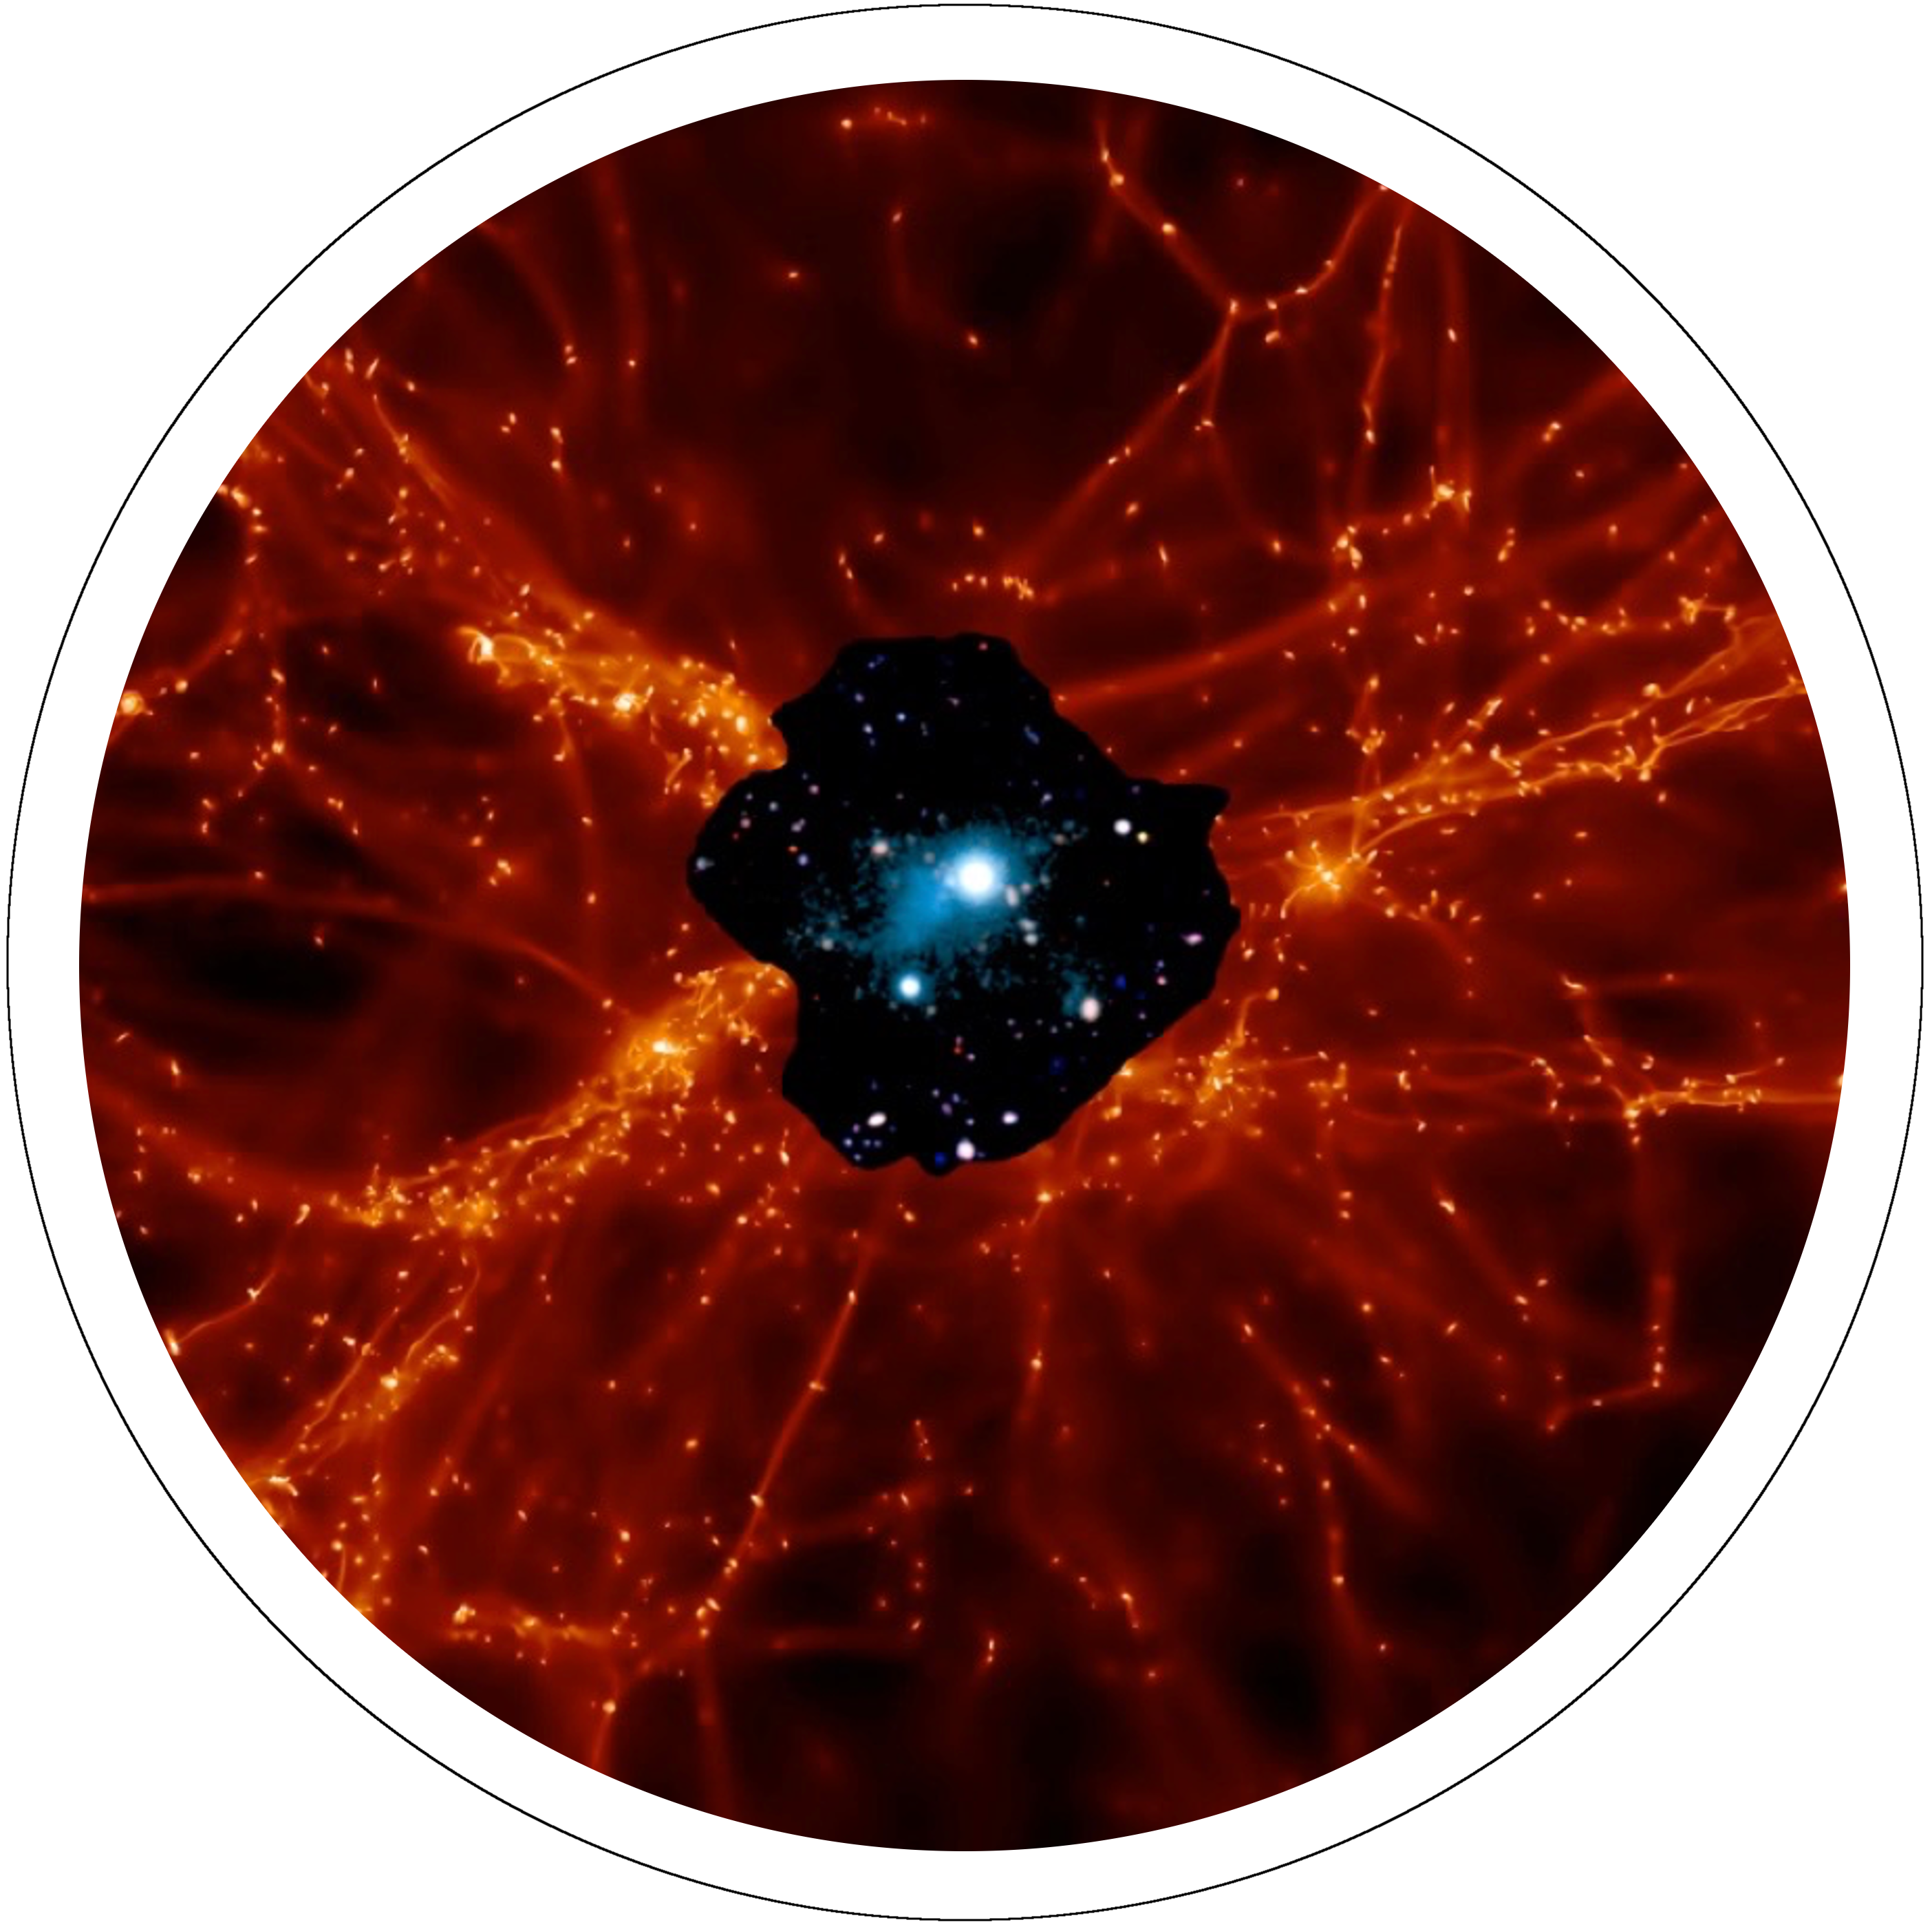
\includegraphics[width=.98\linewidth]{Ly-alpha.png}

          \vspace{1cm}

          {\Large \textbf{Illuminating the Dark Universe}} \\
          {\Large \textbf{with Fluorescent Ly$\symbf{\alpha}$ Emission}} \\
        \end{center}
      \end{minipage}
      \begin{minipage}{0.33\linewidth}
        \begin{center}
          \vspace{2cm}

          {\Large \textbf{The Dark Universe - Mass dominated}} \\
          {\Large \textbf{(Simulation)}}

          \vspace{1cm}

          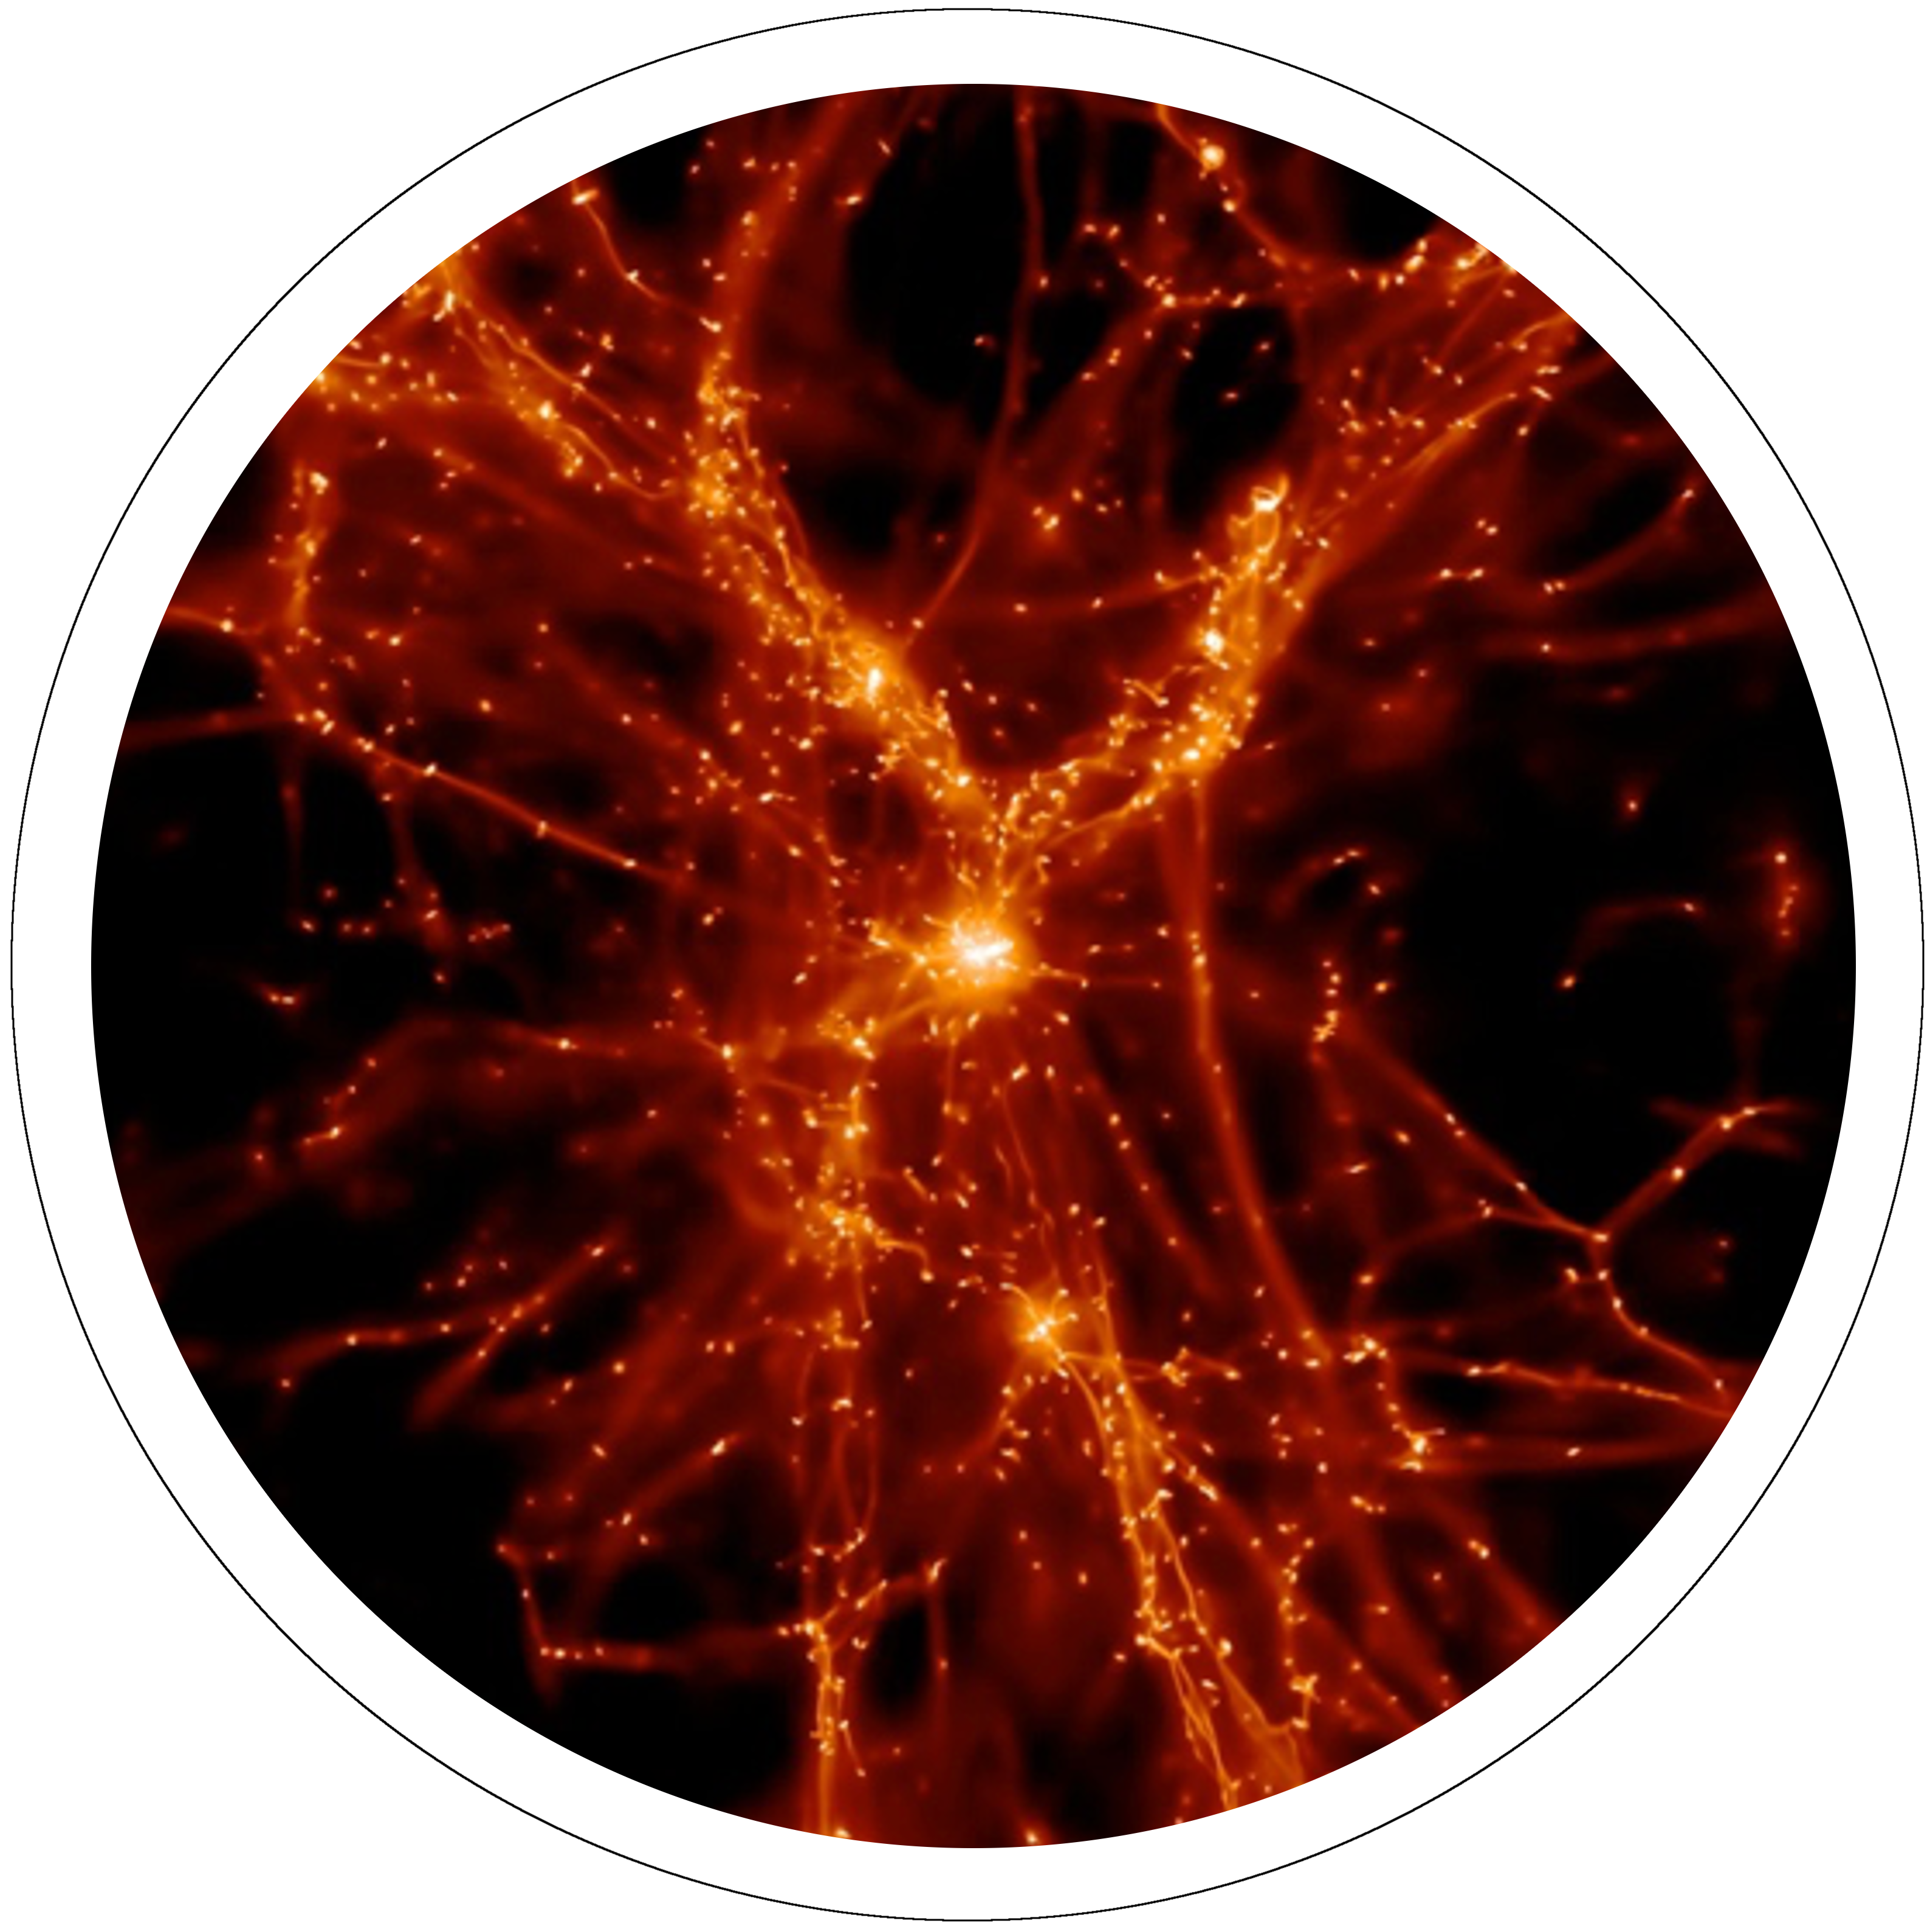
\includegraphics[width=.98\linewidth]{Dark-Universe.png}
        \end{center}
      \end{minipage}
    \end{center}

    % ----------------------------------------------------------------------------
    % BODY
    % ----------------------------------------------------------------------------
    \vspace{2cm}
    \begin{minipage}[t]{0.47\linewidth}

      \begin{gbox}{\textbf{{\LARGE ?}}}{blue1}{}
        \gtxt{{\Large What sets the frequency, size and luminosity of giant
            quasar Nebulae?}}
      \end{gbox}

      \begin{section}{SC}{A Cosmic Web Filament Revealed in Lyman-α Emission around \\
    \hspace*{4cm} a Luminous High-Redshift Quasar}{(Prof. Sebastiano Cantalupo)}
  \begin{minipage}{\linewidth}
    \begin{wrapfigure}{r}{0pt}
      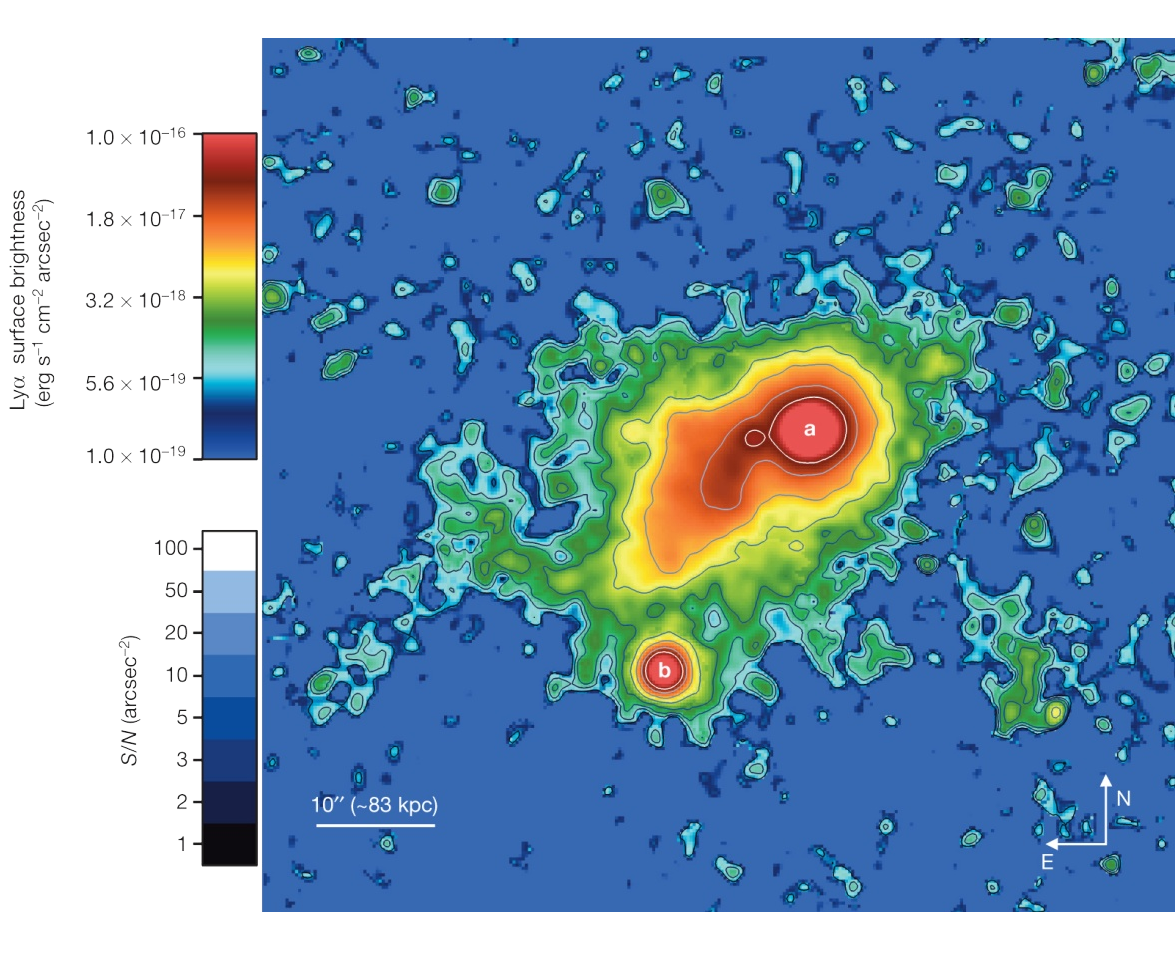
\includegraphics[height=13cm]{SC/Slug.png}
    \end{wrapfigure}
    \strut {\small Simulations of structure formation in the Universe
      predict that galaxies are embedded in a ‘cosmic web’1, where most
      baryons reside as rarefied and highly ionized gas2. This material has
      been studied for decades in absorption against background sources3,
      but the sparseness of these inherently one-dimensional probes preclude
      direct constraints on the three-dimensional morphology of the
      underlying web. Here we report observations of a cosmic web filament
      in Lyman-α emission, discovered during a survey for cosmic gas
      fluorescently illuminated by bright quasars4, 5 at redshift z ≈ 2.3.
      With a linear projected size of approximately 460 physical
      kiloparsecs, the Lyman-α emission surrounding the radio-quiet quasar
      UM 287 extends well beyond the virial radius of any plausible
      associated dark-matter halo and therefore traces intergalactic gas.
      The estimated cold gas mass of the filament from the observed
      emission—about 1012.0 ± 0.5/C1/2 solar masses, where C is the gas
      clumping factor—is more than ten times larger than what is typically
      found in cosmological simulations5, 6, suggesting that a population of
      intergalactic gas clumps with subkiloparsec sizes may be missing in
      current numerical models.}
  \end{minipage}

  \vspace{0.7cm}

  {\footnotesize \textit{[Cantalupo et al. 2017, 2014Natur.506...63C]}}
\end{section}

      \begin{gbox}{\textbf{{\LARGE ?}}}{blue1}{}
        \gtxt{{\Large Are galaxies connected by a filamentary "Cosmic Web"?}}
      \end{gbox}

      \begin{section}{SG}{Stacking the Cosmic Web in Fluorescent Lyman alpha Emission}
  \begin{minipage}[l]{\textwidth}

    {\small Most of the matter in the Universe seems to be distributed along
      filaments connecting galaxies. Fluorescently illuminated by the light of
      first stars and quasars, their expected surface brightness (SB) in
      Lyalpha is beyond current observational limits. By using the deepest
      MUSE/VLT data available, we perform a stacking analysis around Lyalpha
      emitting galaxies (LAEs) between 3<z<4, with orientations determined by
      neighbouring galaxies, reaching a SB sensitivity level bellow the
      predicted signal. No detectable emission is found on intergalactic
      scales implying most of our selected regions do not contain filaments
      given our adopted model. On the other hand, significant emission is
      found on the circum-galactic medium in the direction of the neighbours,
      suggesting typically larger gas densities on those directions. The
      signal is increased around galaxies with a larger number of neighbours
      but seems independent of any other galaxy properties such as redshift,
      neighbour distance and luminosity.}
  \end{minipage}

  \vspace{0.5cm}

  \begin{minipage}{\linewidth}
    \begin{center}
      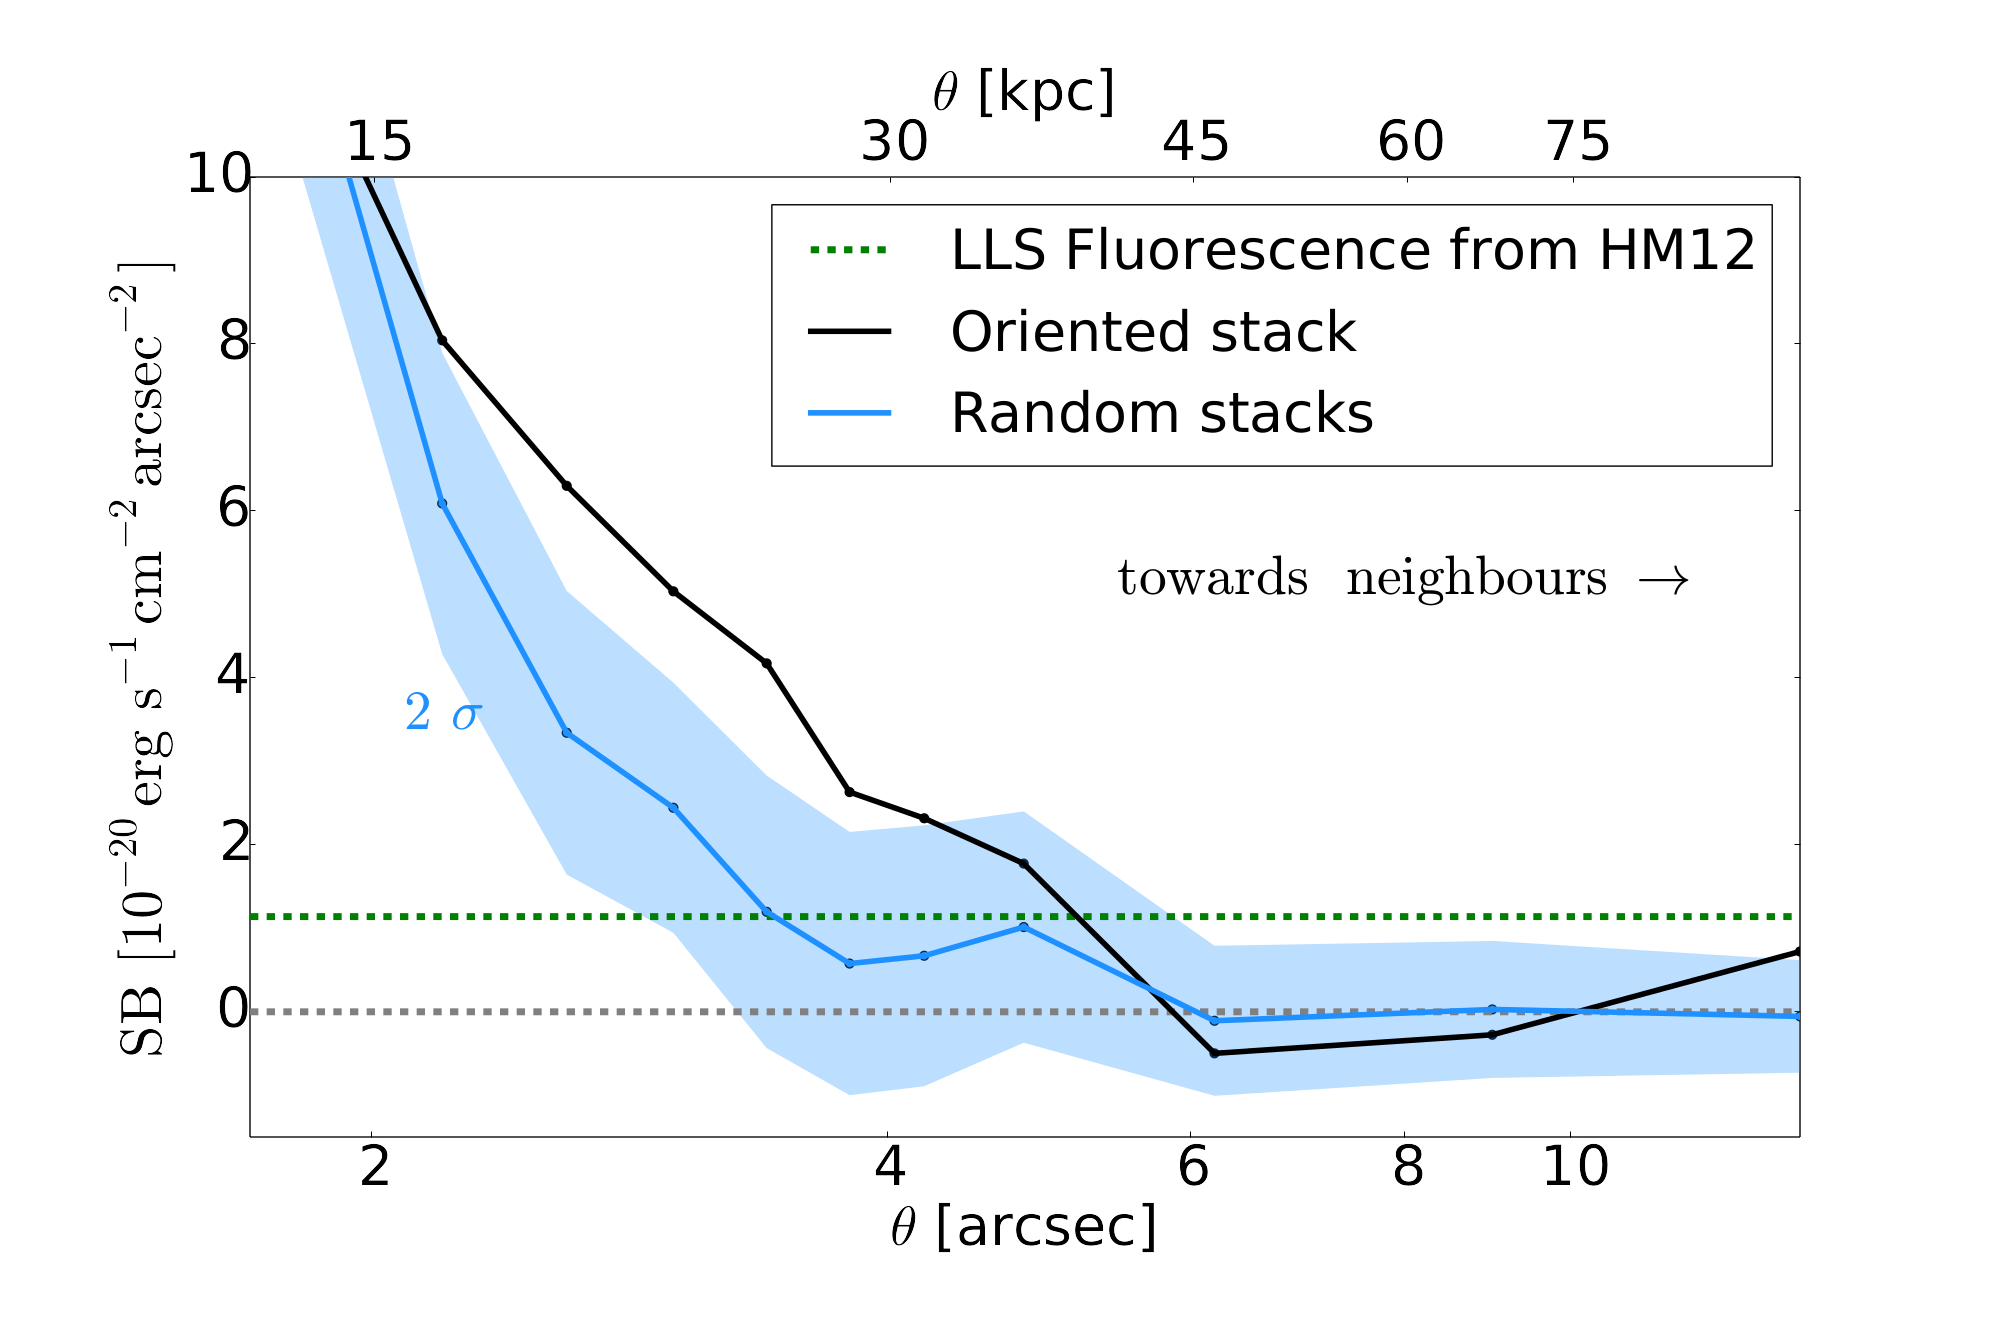
\includegraphics[height=10cm]{SG/SB_right_nmin8.png}
      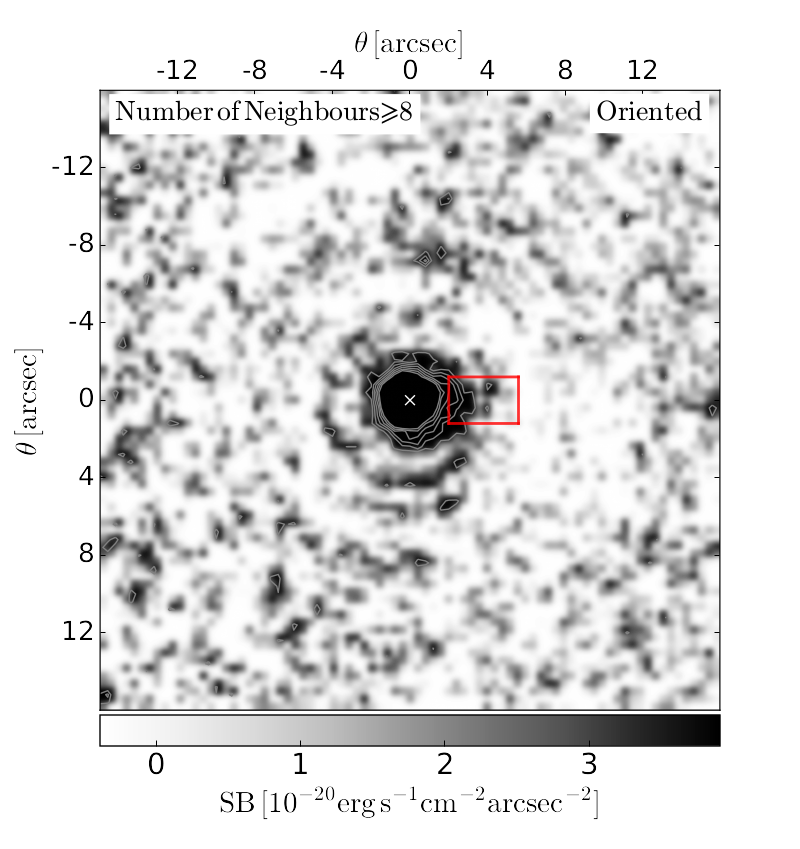
\includegraphics[height=10cm]{SG/stack-nmin8.png}
    \end{center}
  \end{minipage}

  \vspace{0.5cm}

  {\footnotesize \textit{[Gallego, Sofia G. et al. 2017, arXiv:1706.03785]}}
\end{section}

    \end{minipage}
    \hfill
    \begin{minipage}[t]{0.47\linewidth}

      \begin{section}{GP}{Constraining Feedback Models based on the Number of Baryons \\
   \hspace*{4cm} in the Circumgalactic Medium (CGM)}{(Dr. Gabriele Pezzulli, Post-Doc)}
  \begin{minipage}{\linewidth}
    \begin{wrapfigure}{r}{0pt}
      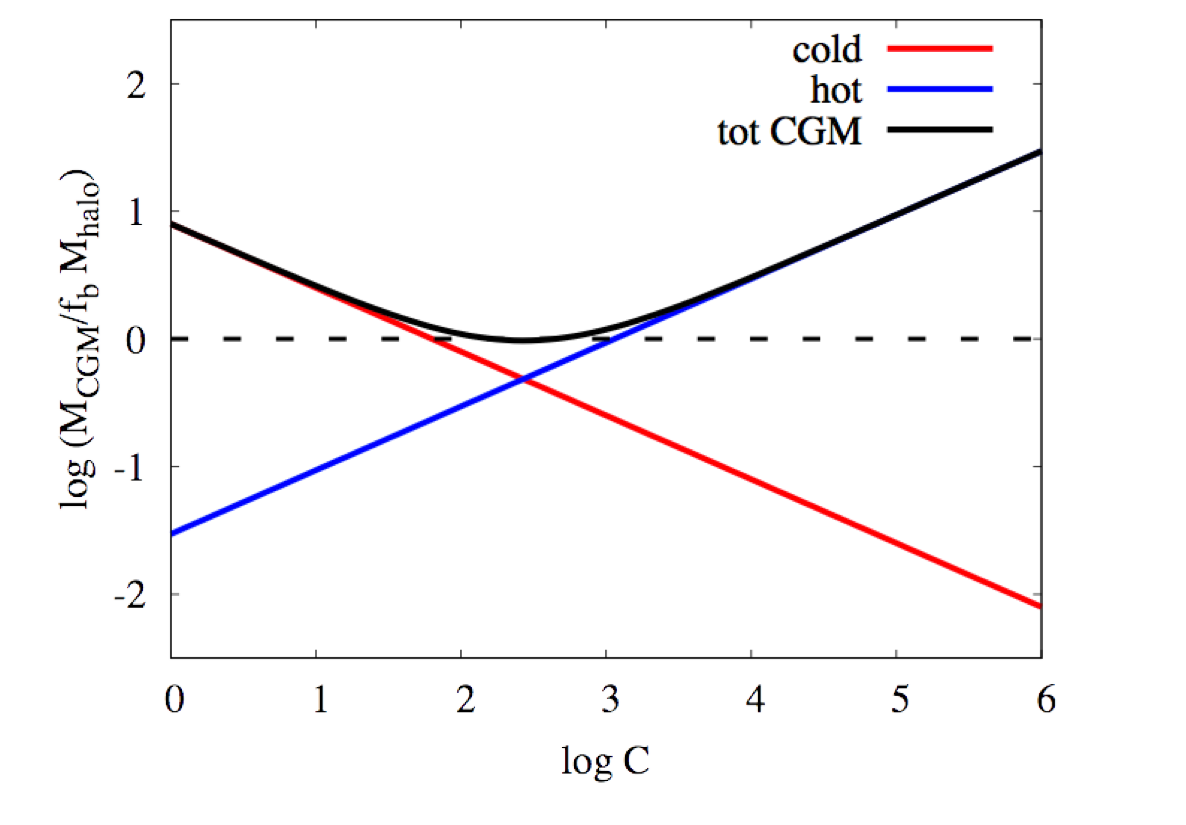
\includegraphics[width=15cm]{GP/fig1.png}
    \end{wrapfigure}
    \strut {\small Here is shown the mass of the CGM in our model of the MUSE
      Giant Ly$\alpha$ nebulae as a function of the clumping factor of the cold
      gas. The mass is in units of the maximum baryon mass
      $(\Omega_b/\Omega_m)M_h$, marked as a horizontal dashed line and the
      fiducial values assumed for halo mass and cold gas temperature are $M_h =
      10^{12.3} M_{\odot}$ and $T=2 \times 10^4 K$. The red, blue and black
      lines are for the cold, hot and total gas, respectively. From this follows
      that viable models require a clumping factor $C \approx 300$ and a total
      baryon fraction very close to the cosmological value.}
  \end{minipage}

  \vspace{0.7cm}

  \begin{minipage}{\linewidth}
    \begin{wrapfigure}{r}{0pt}
      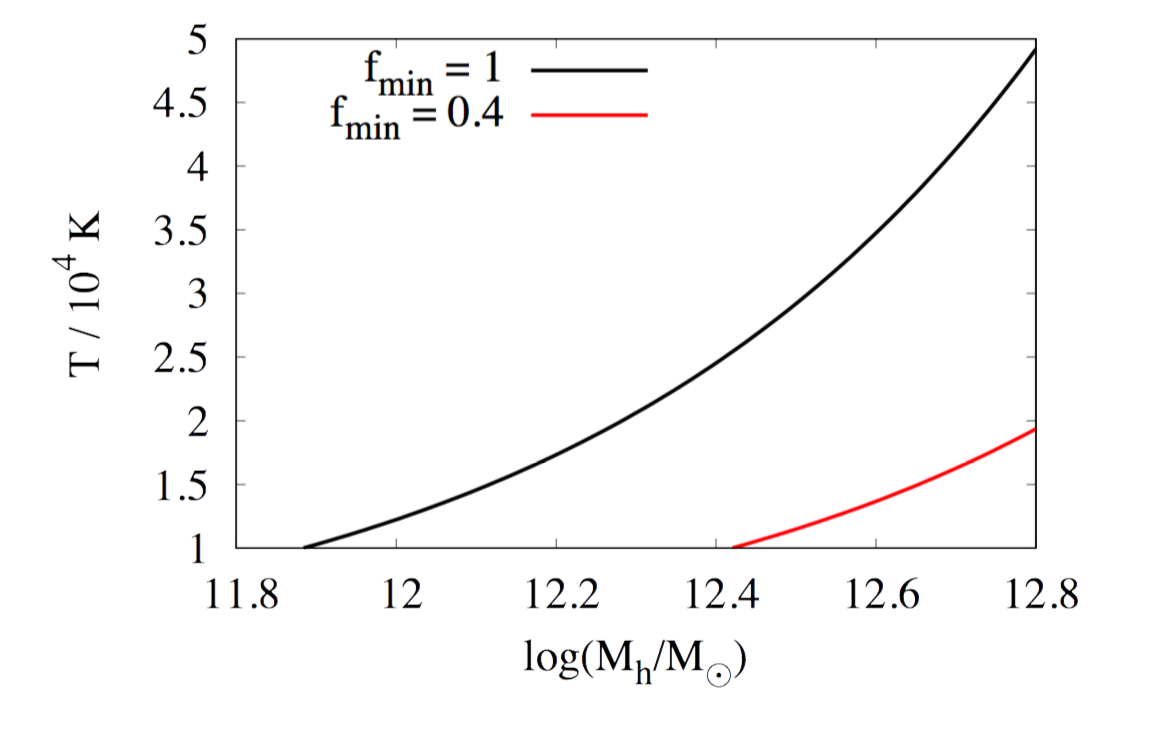
\includegraphics[width=15cm]{GP/fig2.png}
    \end{wrapfigure}
    \strut {\small Shown in the bottom figure is the minimum total CGM baryon
      fraction (corresponding to equipartition of the the CGM into the cold and
      hot phases), as a function of the two model parameters: halo mass and
      temperature of the cold gas. Low halo masses and high temperatures are
      inconsistent with cosmology for exceeding the universal baryon fraction.
      Only the highest halo masses and the lowest gas temperatures are
      consistent with $f_{CGM} \leq 0.4$, as expected for models with strong ejective
      feedback at high $z$.}
  \end{minipage}
\end{section}

      \begin{gbox}{\textbf{{\LARGE ?}}}{blue1}{}
        \gtxt{{\Large What is the origin of the CGM clumps?}}\\
        \gtxt{{\Large Is the CGM multiphase?}}
      \end{gbox}

      \begin{section}{ACE}{}
  \begin{minipage}{\linewidth}
    \begin{wrapfigure}{r}{0pt}
      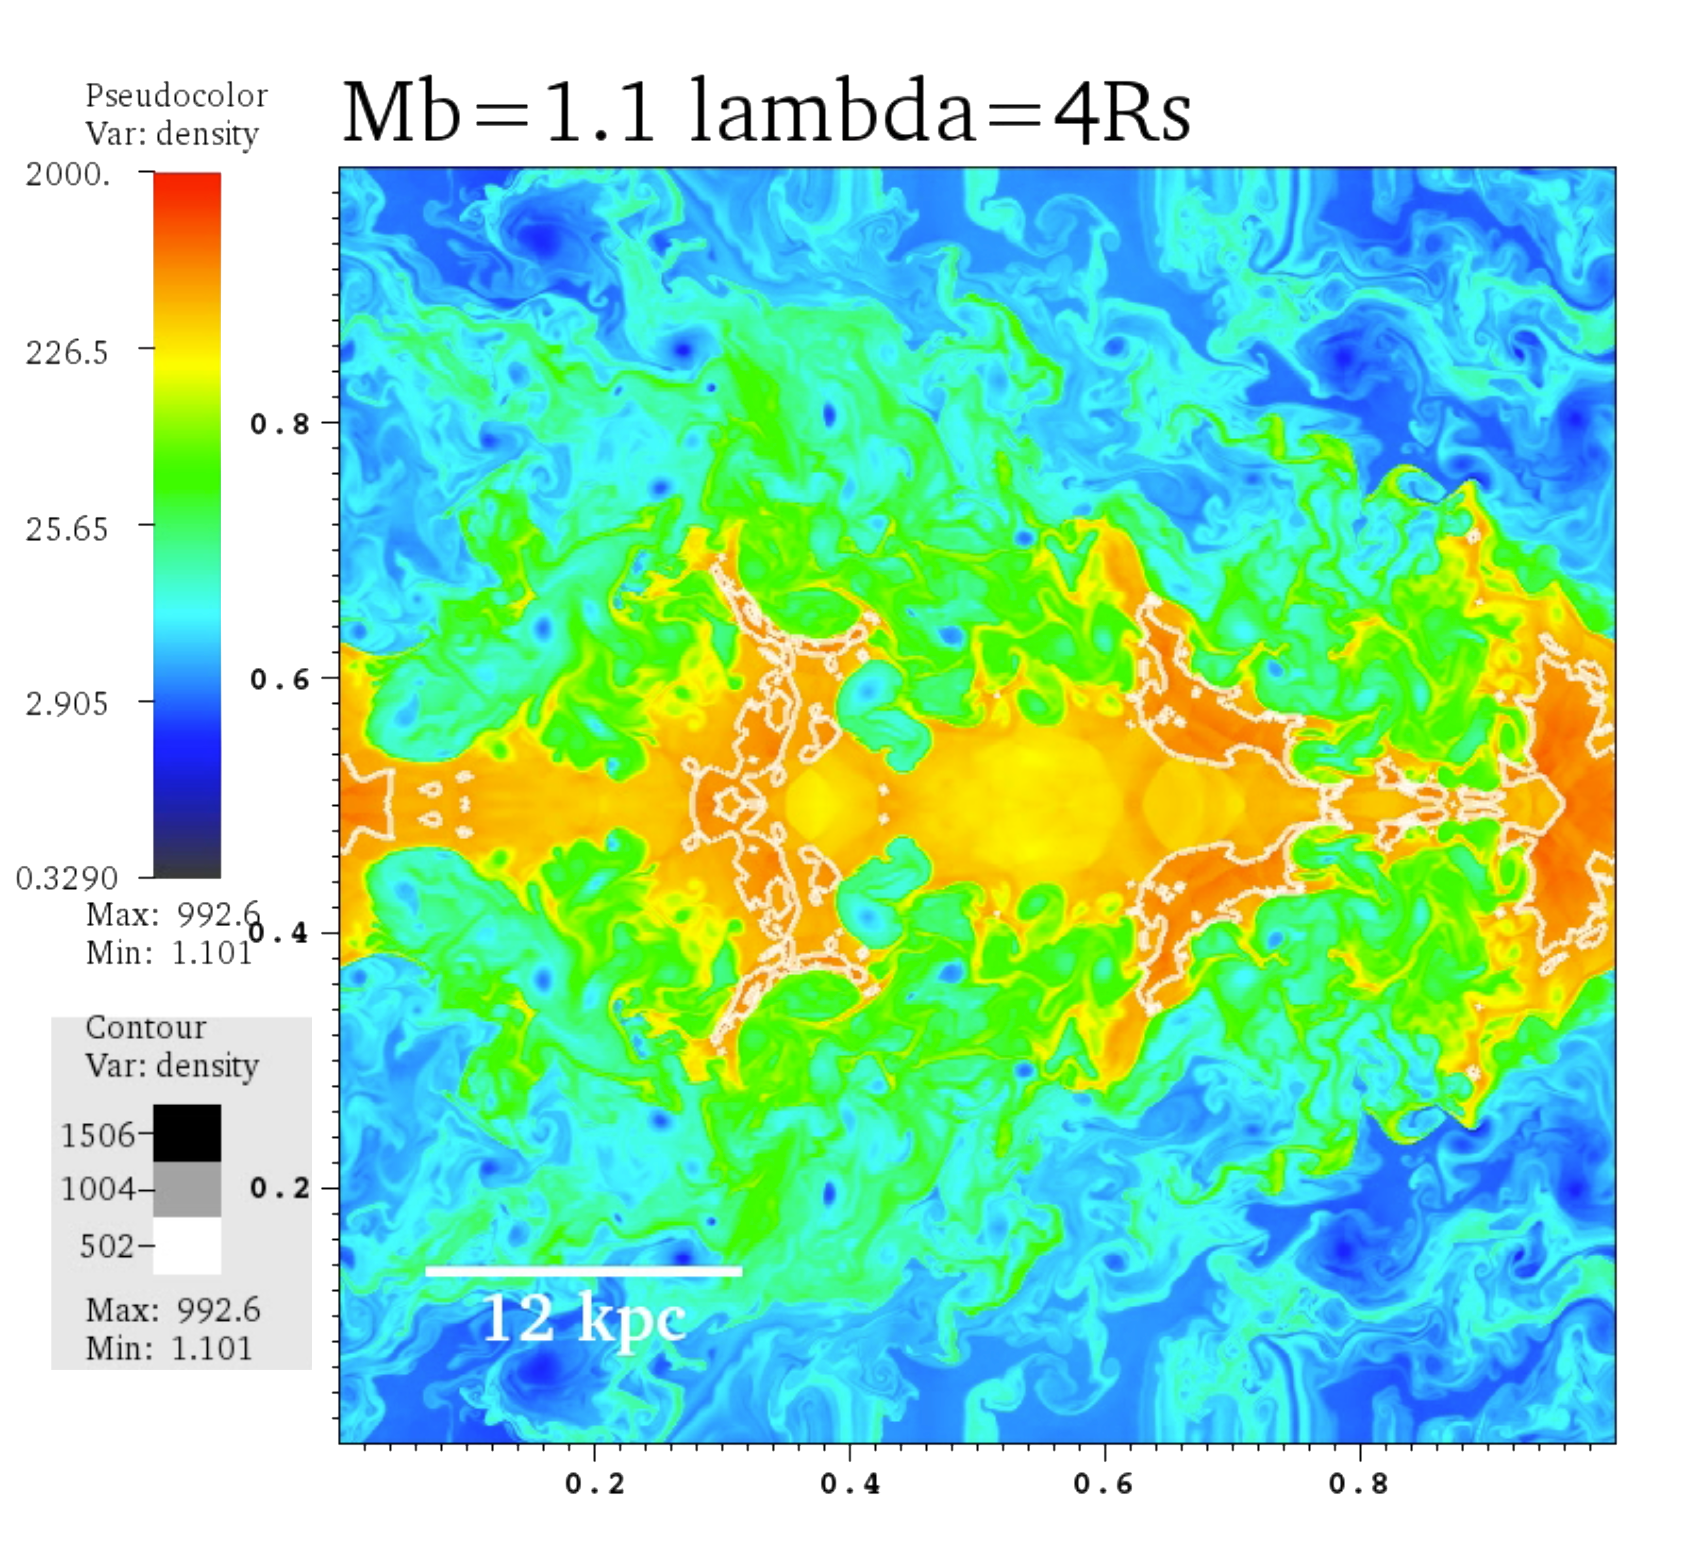
\includegraphics[height=13cm]{ACE/Ramses-2.png}
    \end{wrapfigure}
    \strut {\small Lorem Ipsum is simply dummy text of the printing and
      typesetting industry. Lorem Ipsum has been the industry's standard dummy
      text ever since the 1500s, when an unknown printer took a galley of type
      and scrambled it to make a type specimen book. It has survived not only
      five centuries, but also the leap into electronic typesetting, remaining
      essentially unchanged. It was popularised in the 1960s with the release of
      Letraset sheets containing Lorem Ipsum passages, and more recently with
      desktop publishing software like Aldus PageMaker including versions of
      Lorem Ipsum.}
  \end{minipage}

  \vspace{0.5cm}

  \begin{minipage}{\linewidth}
    \begin{center}
      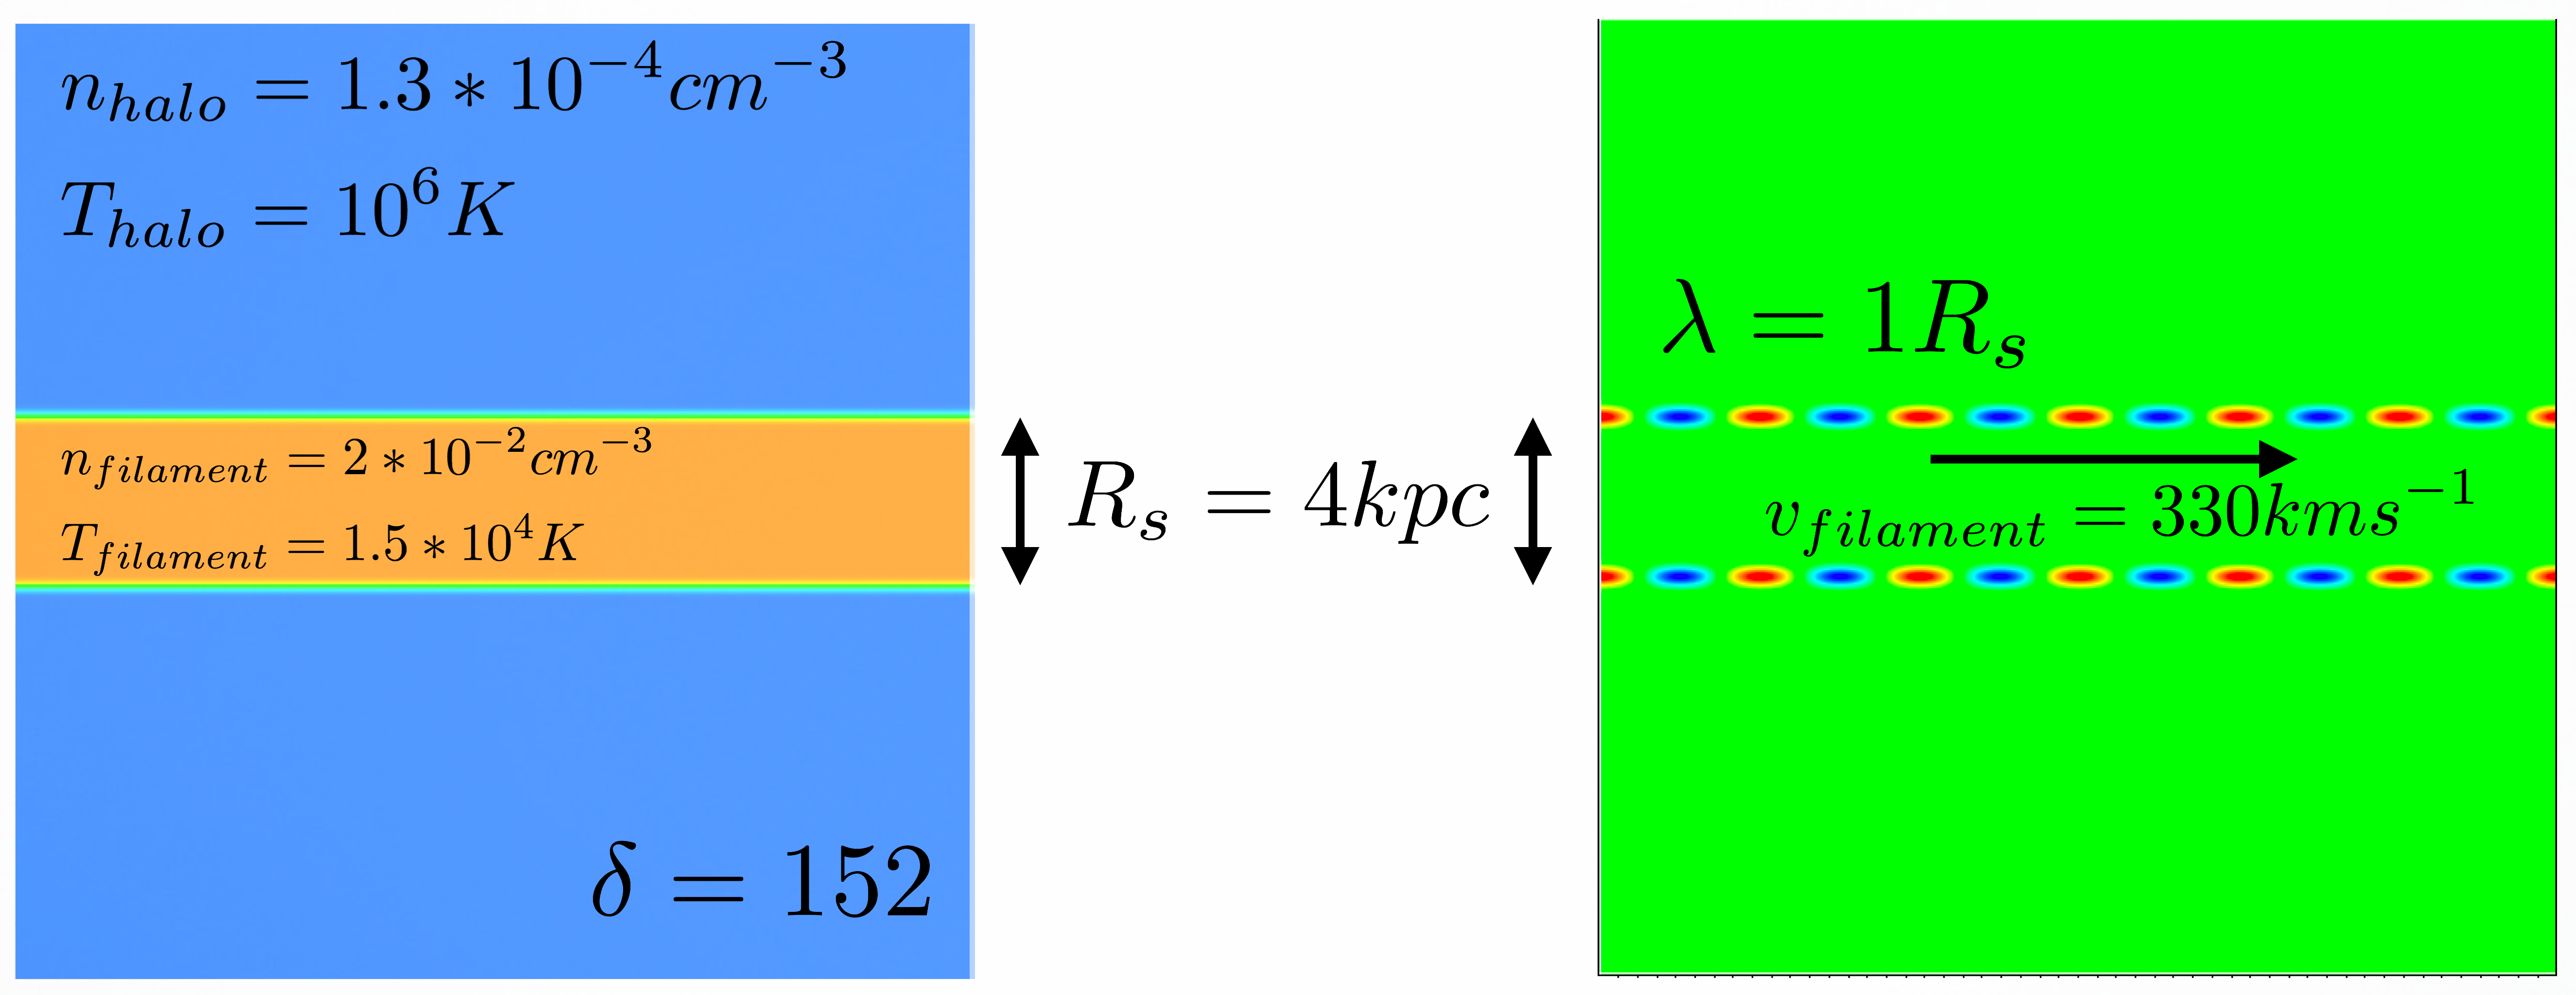
\includegraphics[height=10cm]{ACE/init.png}
    \end{center}
  \end{minipage}
\end{section}

    \end{minipage}
  \end{minipage}
\end{center}


\newpage


% ------------------------------------------------------------------------------
%	HEADER BAR
% ------------------------------------------------------------------------------
\begin{center}
  \begingroup\setlength{\fboxsep}{1cm}\colorbox{Norway4}{
    \begin{tabular}{L{0.29\textwidth} R{0.62\textwidth}}
      
\includegraphics[width=7cm]{eth_logo.png}
      & \mr{2}{{\Large \textbf{\wtxt{``Cosmic Structure Formation Group''}}}} \\

      \wtxt{Department of Physics} & \\

      \wtxt{Institute for Particle Physics and Astrophysics}
      & \wtxt{Group leader: Prof. Dr. Sebastiano Cantalupo} \\
    \end{tabular}
  }\endgroup
\end{center}

\begin{center}
  \begin{minipage}{0.9\linewidth}
    % ----------------------------------------------------------------------------
    % BODY
    % ----------------------------------------------------------------------------
    \vspace{2cm}
    \begin{minipage}[t]{0.47\linewidth}

      \begin{gbox}{}{grey1}{\hspace*{4cm}{\large \textbf{Multi-Unit Spectroscopy
        Explorer (MUSE)}}}
  \begin{minipage}{\linewidth}
    \begin{wrapfigure}{r}{0pt}
      \includegraphics[width=15cm]{MUSE/MUSE.png}
    \end{wrapfigure}
    \strut {\small MUSE is a second
      generation instrument in development for the Very Large Telescope (VLT) of
      the European Southern Observatory (ESO). MUSE couples the
      discovery potential of an imaging device to the measuring capabilities of
      a spectrograph, while taking advantage of the increased spatial resolution
      provided by adaptive optics. This makes it a unique and powerful tool for
      discovering objects that cannot be found in imaging surveys.}
  \end{minipage}

  \begin{minipage}{\linewidth}
    \begin{wrapfigure}{l}{0pt}
      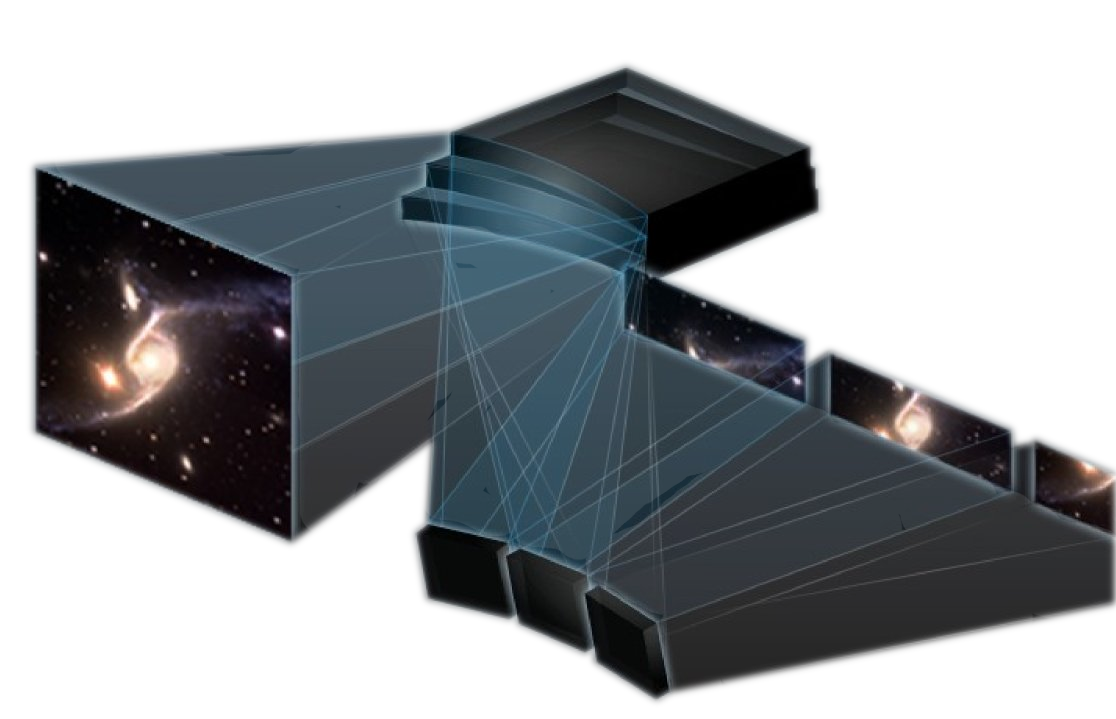
\includegraphics[width=10cm]{MUSE/MUSE_slicer_schematic.png}
    \end{wrapfigure}
    \strut {\small The concept of MUSE foresees the splitting of the adaptive
      optics corrected field of view in 24 sub-fields. Each of these sub-fields
      is fed into a spectrograph (called Integral Field Unit, IFU). An image
      slicer in front of each IFU serves as entrance slit, thus producing a
      spatially resolved spectrum of the full sub-field (from ESO
      website).}
  \end{minipage}

  \vspace{2cm}

  \begin{minipage}{\linewidth}
    \begin{center}
      
\includegraphics[height=3cm]{MUSE/logos.png}
    \end{center}
  \end{minipage}
\end{gbox}

      \begin{gbox}{\textbf{{\LARGE ?}}}{blue1}{}
        \gtxt{{\Large How is gas converted into stars? Is there a dark galaxy
            phase?}}
      \end{gbox}

      \begin{section}{RM}{Dark Galaxy Candidates at Redshift ~3.5 Detected with MUSE}
  \begin{minipage}[l]{\textwidth}

    {\small Recent theoretical models suggest that the early phase of galaxy
      formation involves an epoch when galaxies are gas-rich but inefficient
      at forming stars: a ``dark galaxy'' phase. We perform an integral field
      survey for dark galaxies fluorescently illuminated by quasars at z>3
      with MUSE, which provides us a nearly uniform sensitvity coverage over a
      large volume in redshift space, compared to previous narrow-band imaging
      surveys. By comparing the rest-frame equivalent width (EW\_0)
      distributions of the Lyalpha sources detected in proximity to the
      quasars and in control samples, we detect a clear correlation between
      the locations of high EW\_0 objects and the quasars, not seen in other
      properties such as Lyalpha luminosities or volume overdensities,
      suggesting the possible fluorescent nature of at least some of these
      objects. Among these, we found 6 dark galaxy candidates with EW\_0 limits
      larger than 240 Angstrom with similar properties to previously detected
      candidates at z~2.4. Our results also provide a lower limit of 60 Myr on
      the quasar lifetime.}
  \end{minipage}

  \vspace{0.5cm}

  \begin{minipage}{\linewidth}
    \begin{center}
      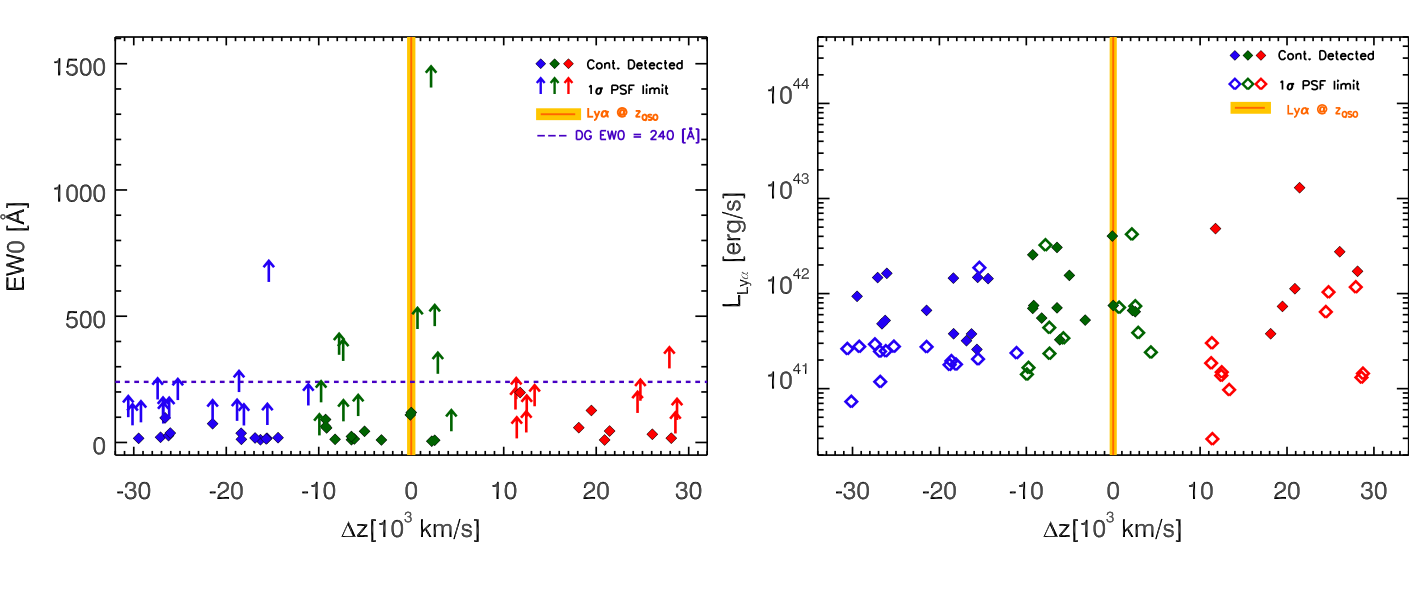
\includegraphics[height=10cm]{RM/EW_LUM_highz.png}
    \end{center}
  \end{minipage}

  \vspace{0.5cm}

  {\footnotesize \textit{[Marino, Raffaella Anna et al. 2017, arXiv:1709.03522]}}
\end{section}
      \begin{section}{SS}{Incorporating the Cosmological Radiative Transfer code, \\
    \hspace*{4cm} RADAMESH with Hydrodynamics}{(Saeed Sarpas, PhD)}
  \begin{minipage}{\linewidth}
    \strut {\small The advent of supercomputers and the more efficient CPU
      architectures has enabled cosmologists to simulate the Universe in more
      detail. So far, Gravity, Hydrodynamics and radiative cooling and heating
      effects have been included into the cosmological simulations, however
      still some important parts of the puzzle (such as
      proper stellar and AGN feedback mechanisms, magneto-hydrodynamics and
      radiative transfer effects) are either missing or not fully implemented.
      In the era of high precision cosmology, adding these extra phenomena to
      cosmological simulation seems crucial,
      especially to reach the percent accurate results. Our objective is to
      incorporate cosmological simulations with radiative transfer effects.
      Presently, these effects are treated in a post-processing state.
      Considering the active role of radiative hydrodynamics in cosmic structure
      formation, post-processing these effects might lead to less accurate
      results. The
      non-local nature of these effects make them extremely tricky and
      challenging to be implemented in an efficient way. We accept this
      challenge with the expectation of getting more precise results especially
      in the environment of our interest which is circumgalactic medium
      (CGM) illuminated by a bright quasar.\\
      The pictures show how a bright quasar is able to ionize its
      environment in a comparably short period of time (here the interval
      between two snapshots is less than 100000 yrs). This
      result has been generated by post-processing an EAGLE snapshot at $z
      \approx 3$ using RADAMESH code.
    }
  \end{minipage}

  \vspace{0.5cm}

  \begin{minipage}{\linewidth}
    \begin{center}
      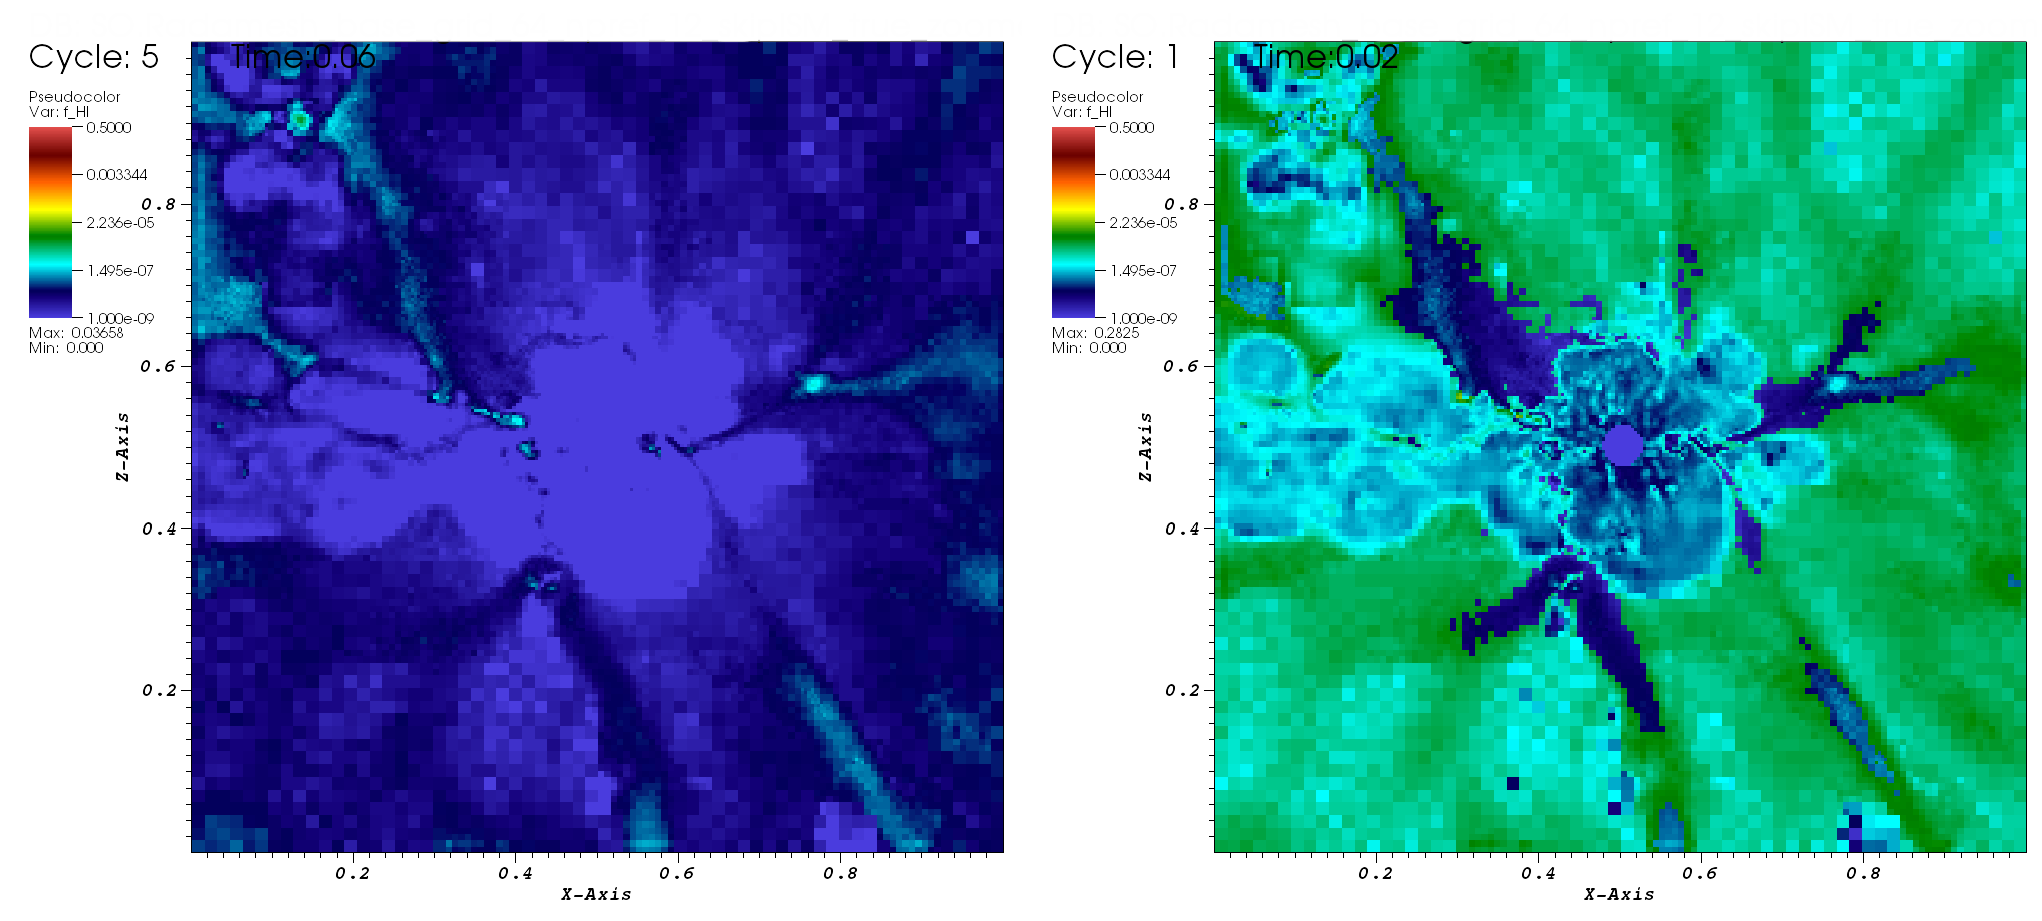
\includegraphics[height=10cm]{SS/QSO.png}
    \end{center}
  \end{minipage}
\end{section}

    \end{minipage}\hfill
    \begin{minipage}[t]{0.47\linewidth}

      \begin{section}{SC}{RADAMESH: Cosmological Radiative Transfer for Adaptive Mesh\\
    \hspace*{4cm} Refinement Simulations}{(Prof. Sebastiano Cantalupo)}
  \begin{minipage}[l]{\textwidth}

    {\small RADAMESH is a three-dimensional radiative transfer (RT) code, based
      on a ray-tracing, photon-conserving and adaptive (in space and time)
      scheme. It uses a novel Monte Carlo approach to sample the radiation field
      within the computational domain on a ”cell-by-cell” basis. Thanks to this
      algorithm, the computational efforts can be focused where needed most,
      i.e. within the Ionization-fronts (I-fronts). This results in an increased
      accuracy level and a huge gain in computational speed with respect to a
      ”classical” Monte Carlo RT, especially when combined with an Adaptive Mesh
      Refinement (AMR) scheme. RADAMESH is able to adaptively refine the
      computational mesh in correspondence of the I-fronts, allowing to fully
      resolve them within large, cosmological boxes. The propagation of ionizing
      radiation is followed from an arbitrary number of sources and from the
      recombination radiation produced by H and He. The chemical state of six
      species (HI, HII, HeI, HeII, HeIII, e) and gas temperatures are computed
      with a time-dependent, non-equilibrium chemistry solver. Using our AMR
      scheme, we find that properly resolving the I-front of a bright quasar
      during Reionization produces a large increase of the predicted gas
      temperature within the whole HII region.}
  \end{minipage}

  \vspace{0.5cm}

  \begin{minipage}{\linewidth}
    \begin{center}
      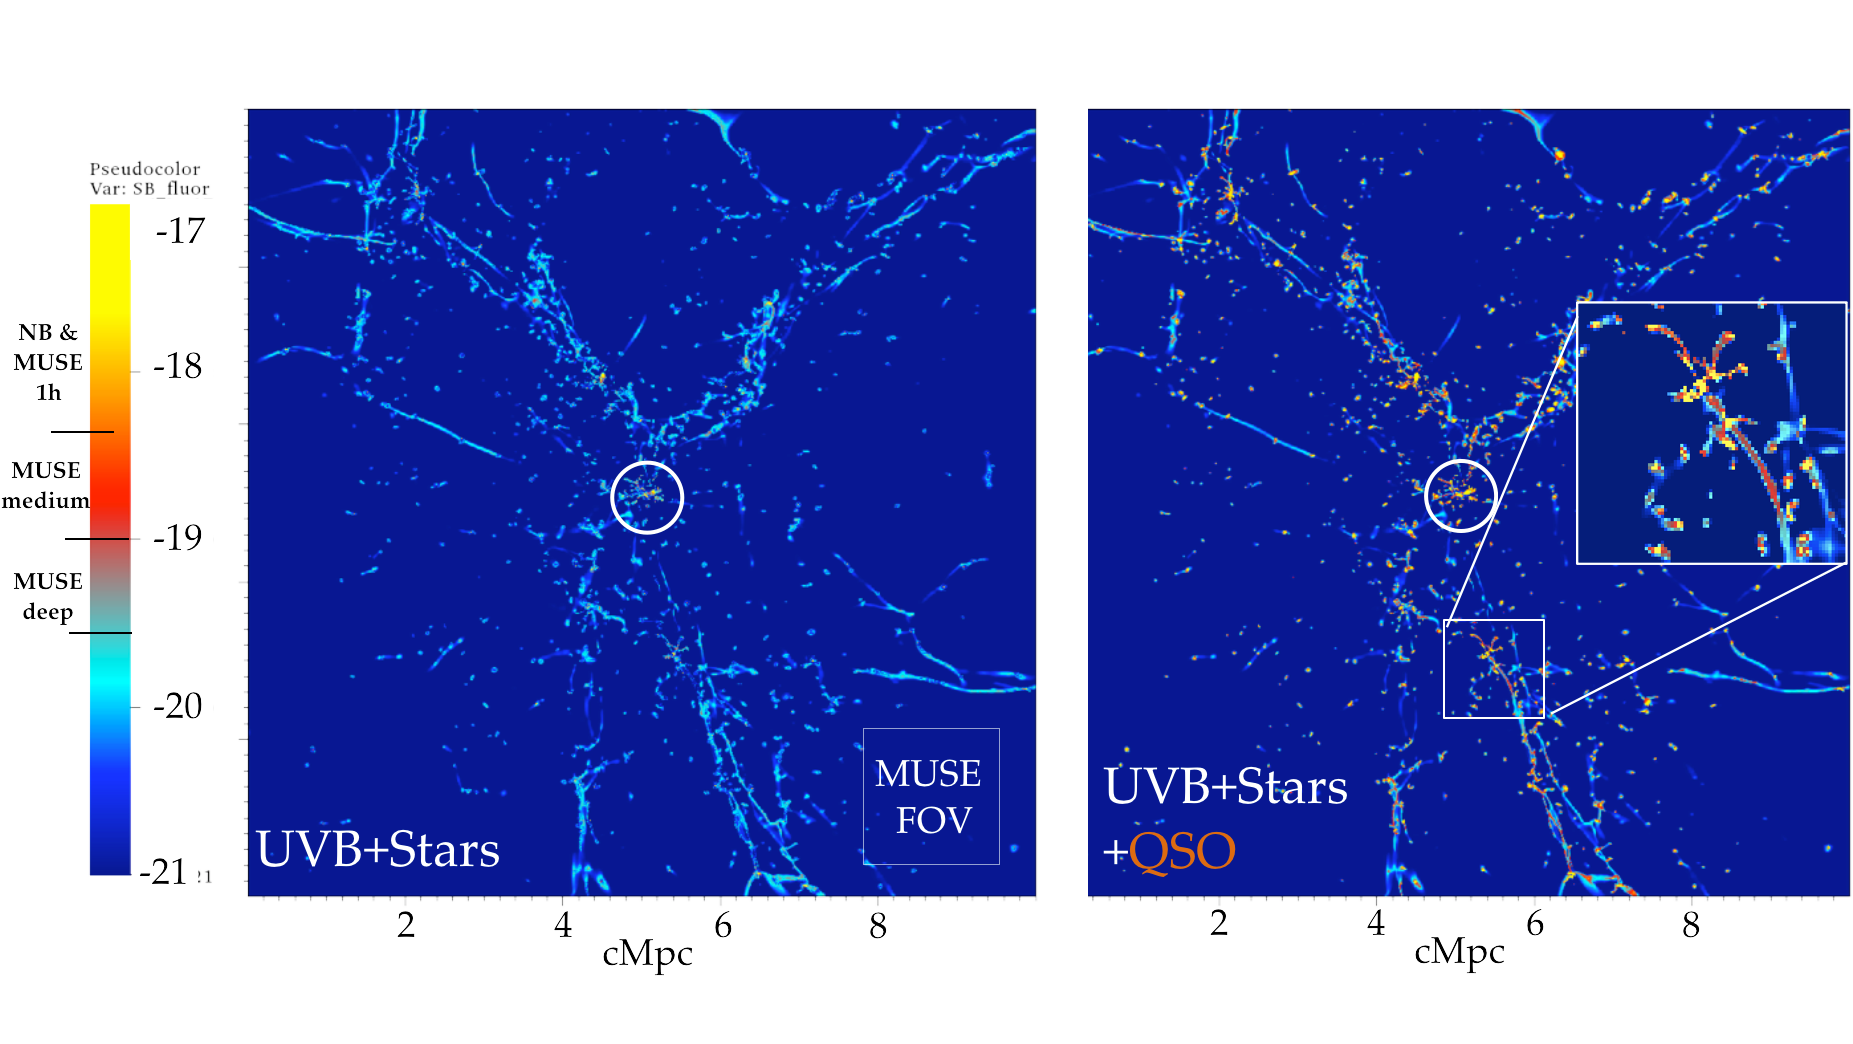
\includegraphics[height=15cm]{SC/Radamesh.png}
    \end{center}
  \end{minipage}

  \vspace{0.5cm}

  {\footnotesize \textit{[Cantalupo \& Porciani 2011, 2011MNRAS.411.1678C]}}
\end{section}

      \begin{gbox}{\textbf{{\LARGE ?}}}{blue1}{}
        \gtxt{{\Large What is the density distribution of the cold gas in CGM?}}
      \end{gbox}

      \begin{section}{MT}{Analyzing the CGM in the Massive Dark Matter Halos of \\
    \hspace*{4cm} Cosmological Simulations}{(Marius Tresoldi, Master Student)}
  \begin{minipage}{0.52\linewidth}
{\small In order to better understand the high redshift giant
      Ly-$\alpha$ nebulae revealed by MUSE, we analyze the properties of the
      hydrogen gas in the most massive dark matter halos at $z \sim 3$ using
      hydrodynamical simulations of cosmic structure formation such as the EAGLE
      and the Illustris project. These large-scale simulations have boxsizes of
      up to 100 cMpc and thus provide a useful sample of the rare halos of
      interest with $M >10^{12.5} M_{\odot}$. Shown are both the phase diagram and
      the radial
      temperature distribution of the hydrogen gas in the RefL0100N1504
      simulation of EAGLE at $z=3.01$, where one can clearly distinguish between
      two phases. First there is the hot gas at $T \sim 10^{6.5} \mathrm{T}$ which
      corresponds to gas accreted from the intergalactic medium (IGM) that has
      been shock heated while falling into the gravitational potential well of
      the dark matter halo. The second phase is the cold CGM gas at $T \sim
      10^{4.1} \mathrm{T}$ which is assumed to be responsible for the Ly-$\alpha$
      emission observed by MUSE when ionized by a central quasar.}
  \end{minipage}
  \hfill
  \begin{minipage}{0.42\linewidth}
      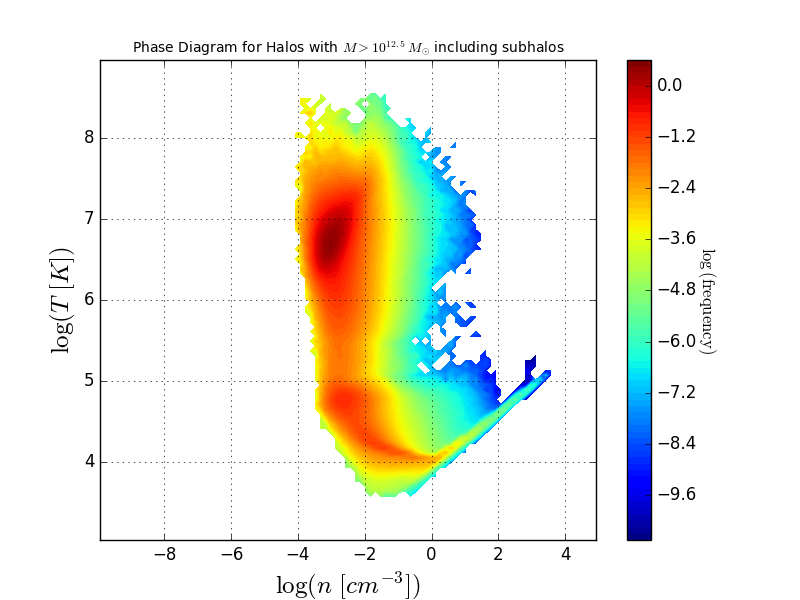
\includegraphics[height=12cm]{MT/PhaseDiagram.png}
      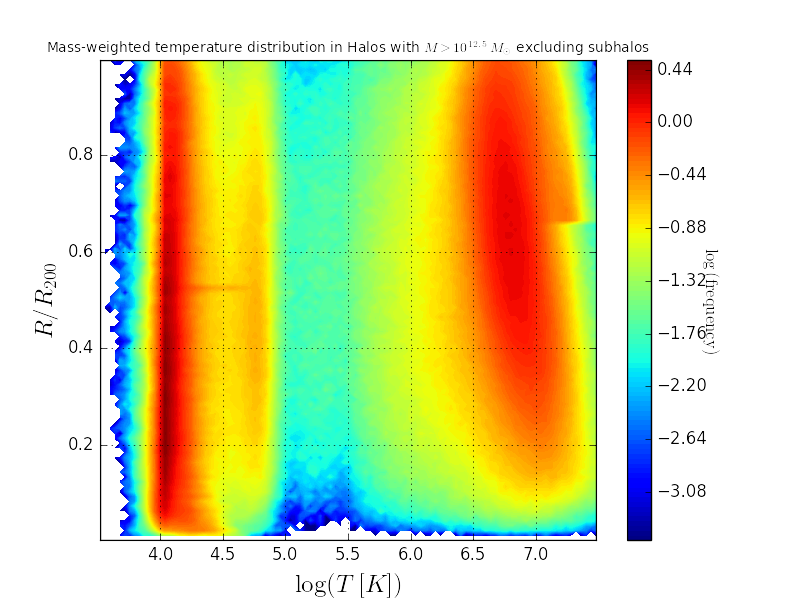
\includegraphics[height=12cm]{MT/T_R_dist.png}
  \end{minipage}
\end{section}


      \begin{gbox}{}{grey1}{}
        \begin{center}
          \vspace{1cm}

          \includegraphics[width=\linewidth]{Group-photo.png}
        \end{center}
      \end{gbox}

    \end{minipage}
  \end{minipage}
\end{center}

\end{document}